\chapter{System wykrywania anomalii}

\begingroup
\leftskip4em
\rightskip\leftskip
\noindent
\textbf{Abstrakt} Rozdział prezentuje powstały system wykrywania anomalii. Wymienia wymagania funkcjonalne oraz niefunkcjonalne postawione przed systemem. Przedstawia technologie wykorzystane w tworzeniu systemu oraz opisuje implementację funkcjonalności
\par
\endgroup

\section{Wytyczne projektowe}
 Uniwersalny system wykrywania anomalii ma za zadanie ułatwić korzystającemu detekcję anomalii dla dowolnego zbioru danych statystycznych. W tym celu najważniejszą funkcją systemu jest automatyzacja wyboru optymalnego modelu detekcji anomalii. System po procesie analizy danych ma wizualizować wynik detekcji w sposób przejrzysty i zrozumiały dla korzystającego.    
\subsection{Wymagania funkcjonalne}
\begin{itemize}
    \item Przesłanie pliku zawierającego zbiór danych w formatach: JSON, CSV
    \item Oczyszczenie danych z brakujących wartości oraz wyskalowanie 
    \item Wybór optymalnego modelu (algorytm i parametry) 
    \item Detekcja anomalii w zbiorze danych z wykorzystaniem wybranego przez system modelu
    \item Utworzenie oczyszczonego zbioru danych z anomalii (wartość anomalności w 99. per centylu)
    \item Utworzenie zbioru danych z wartością anomalności dla każdej obserwacji
    \item Stworzenie raportu z przebiegu i wyniku detekcji anomalii
\end{itemize}
\subsection{Wymagania niefunkcjonalne}
\begin{itemize}
    \item Zbiory danych do pobrania (oczyszczone i zawierające wartość anomalności) powinny być w formacie przesłanych danych
    \item System powinien być jak najbardziej intuicyjny i prosty w obsłudze
    \item Raport powinien zawierać niezbędne informacje potrzebne do dalszej analizy przez użytkownika
    \item System oraz raport powinny być przystępne dla użytkownika bez wiedzy na temat detekcji anomalii
\end{itemize}

\section{Analiza technologiczna}
\subsection{Wykorzystane technologie oraz biblioteki}
System powstał z wykorzystaniem języka programistycznego Python 3.7. Jest to prosty do nauczenia, przejrzysty, a zarazem wszechstronny język programistyczny o rosnącej popularności zwłaszcza w środowisku uczenia maszynowego. Do stworzenia aplikacji webowej wykorzystano mikro-framework Flask 1.1.2. Do projektowania struktury i interfejsu graficznego strony internetowej wykorzystano: HTML, JavaScript oraz biblioteki CSS -- Bootstrap.
Do wyboru optymalnego modelu detekcji anomalii wykorzystano bibliotekę MetaOD, którą opisano w sekcji \ref{sec:MetaOD}. Do detekcji anomalii w zbiorze danych, wykorzystując algorytmy z przestrzeni bazowej modeli, skorzystano z gotowych implementacji algorytmów zawartych w bibliotece PyOD. 
Do analizy oraz przechowywania danych w strukturach danych użyto pakietu Pandas (tabela danych) oraz Numpy(tablice). Do skalowania zbioru danych wykorzystano bibliotekę Scikit-learn. Matplotlib został wykorzystany jako kreator wykresów pudełkowych oraz histogramów.

% Funkcjonalność aplikacji webowej została napisana w języku Python 3.7 z wykorzystaniem frameworku Flask 1.1.2.
% Interfejs graficzny powstała z użyciem języków HTML oraz JavaScript.
% Interfejs graficzny wykorzystuje bibliotekę CSS -- Bootstrap. 
% Do przechowywania danych w strukturach danych wykorzystano biblioteki: NumPy(tablice) oraz Pandas(tabela danych). 
% Detekcje anomalii przeprowadzona została z wykorzystaniem MetaOD i PyOD. 
% Do tworzenia wykresów wykorzystano bibloteki Matplotlib
% % \begin{itemize}
% %     \item Python 3.7 - 
% %     \item HTML
% %     \item Flask
% %     \item Bootstrap - bibloteka CSS, służąca do tworzenia interfejsu graficznego strony internetowej. 
% %     % \item Jinja2 
% %     \item PyOD
% %     \item MetaOD
% %     \item Sklearn
% %     \item FPDF
% %     \item Matplotlib
% %     \item Pandas
% %     \item Numpy
% % \end{itemize}
\subsection{Wykorzystane narzędzia programistyczne}
Zintegrowanym środowiskiem programistycznym wykorzystanym przy tworzeniu aplikacji był PyCharm Professional, czeskiej firmy JetBrains. To zaawansowane i wszechstronne środowisko ułatwia proces pisania kodu źródłowego, testowania oraz rozwijania oprogramowania. Posiada graficzny debugger ułatwiający identyfikację błędów. Wspiera pisanie aplikacji webowych. Posiada integrację z systemem kontroli wersji Git, wykorzystanego przy produkcji systemu do tworzenia kolejnych wersji rozwijanego projektu. Dzięki czemu implementacja nowych funkcjonalności odbywa się bez obawy utraty działającej wersji systemu.

% \section{Architektura systemu}
\section{Implementacja funkcjonalności}

\subsection{Uzyskanie danych}
System rozpoczyna działanie od strony startowej, na której klient może wybrać plik z danymi, które chce poddać zadaniu detekcji anomalii. Plik musi mieć rozszerzenie CSV lub JSON. Po naciśnięciu przycisku ,,Analizuj'' następuje przesłanie pliku do systemu. System sprawdza zgodność rozszerzenia pliku, jeżeli rozszerzenie jest obsługiwane, następuje zapisanie pliku na serwerze.
\begin{figure}
    \centering
    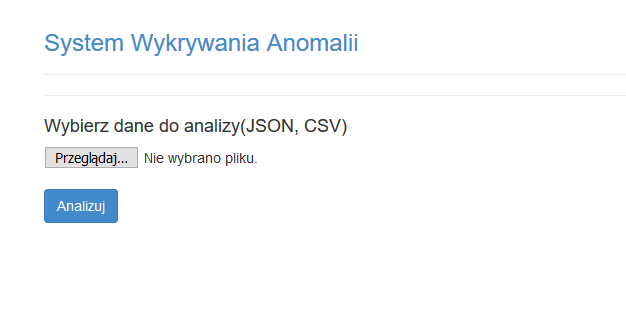
\includegraphics[width=\textwidth]{chapters/projekt/images/index.png}
    \caption{Strona startowa systemu wykrywania anomalii}
    \footnotesize{źródło: Opracowanie własne}
    \label{fig:my_label}
\end{figure}
\subsection{Przygotowanie danych}
Po zapisaniu pliku na serwerze następuje wczytanie danych z wykorzystaniem biblioteki Pandas. Wczytane dane są weryfikowane pod kątem brakujących wartości, jeśli zbiór danych zawiera brakujące wartość, system w miejsce brakującej wartości wstawia średnia z cechy (kolumny). System również dokonuje standaryzacji zbioru danych, wykorzystując funkcje biblioteki Scikit-learn -- \textit{MinMaxScaler}, która skaluje obserwację według wzoru:
\begin{equation}
       X_{std} = \frac{X - X_{min}}{X_{max} - X_{min}} 
\end{equation}
%     % X_{scaled} = X_{std} \cdot (max - min) + min
%  \end{gather}
 gdzie min, max są to minimalne i maksymalne wartości obserwacji. \textit{MinMaxScaler} został wybrany ze względu na największą skuteczność dla zestawu testowych zbiorów danych (podsekcja \ref{minimen}).
%  % \begin{sidewaystable}
%     \centering
\begin{table}[]
    \centering
\begin{tabularx}{\textwidth}{lXXXXX}
      Zbiór & Dane oryginalne & Robust Scaler & Standard Scaler & MinMax Scaler & Power Transformer \\ \hline
arrhythmia &               0.7480 &                  0.7527 &            0.7685 &      0.8093 &      0.7619 \\
    cardio &               0.5474 &                  0.6150 &            0.8604 &      0.9109 &      0.3830 \\
     glass &               0.6249 &                  0.4016 &            0.7122 &      0.7518 &      0.6076 \\
ionosphere &               0.8336 &                  0.8308 &            0.8065 &      0.8678 &      0.8481 \\
    letter &               0.8790 &                  0.8096 &            0.8976 &      0.8411 &      0.9062 \\
    lympho &               0.9977 &                  0.9930 &            0.9953 &      0.9941 &      1.0000 \\
      musk &               0.9460 &                  0.9994 &            0.7267 &      0.9923 &      0.1024 \\
 optdigits &               0.7431 &                  0.4615 &            0.5380 &      0.4757 &      0.4856 \\
 pendigits &               0.6975 &                  0.7786 &            0.6792 &      0.7218 &      0.5707 \\
      pima &               0.6996 &                  0.7025 &            0.5650 &      0.6751 &      0.4289 \\
 satellite &               0.5549 &                  0.5394 &            0.6123 &      0.6380 &      0.3594 \\
satimage-2 &               0.9795 &                  0.9715 &            0.9688 &      0.9808 &      0.9469 \\
 vertebral &               0.3771 &                  0.7484 &            0.3465 &      0.2254 &      0.2835 \\
    vowels &               0.9551 &                  0.9727 &            0.9551 &      0.9543 &      0.9781 \\
       wbc &               0.8980 &                  0.8844 &            0.9689 &      0.8814 &      0.6293 \\
     mnist &               0.7737 &                  0.8051 &            0.6330 &      0.8130 &      0.6960 \\
   shuttle &               0.6166 &                  0.9860 &            0.6167 &      0.9973 &      0.6105 \\
\hline
Średnia &0.7572&
0.7795&
0.7442&
0.7959&
0.6234
\end{tabularx}
\caption{Porównanie skuteczności modelu wybranego przez MetaOD w zależności od metody standaryzacji danych -- pole pod krzywą ROC}
\footnotesize{źródło: Opracowanie własne}
\label{tab:roc_sc}
\end{table}
% \end{sidewaystable}
\begin{sidewaystable}
    \centering
\begin{tabular}{lrrrrr}
      Zbiór & Dane oryginalne & RobustScaler & StandardScaler & MinMaxScaler & PowerTransformer \\ \hline
arrhythmia &               0.3788 &                  0.4545 &            0.3788 &      0.4697 &      0.4242 \\
    cardio &               0.2273 &                  0.2159 &            0.4489 &      0.5114 &      0.1307 \\
     glass &               0.1111 &                  0.2222 &            0.1111 &      0.1111 &      0.0000 \\
ionosphere &               0.6349 &                  0.6429 &            0.6032 &      0.6984 &      0.6349 \\
    letter &               0.3800 &                  0.2600 &            0.5400 &      0.3100 &      0.4800 \\
    lympho &               0.8333 &                  0.6667 &            0.8333 &      0.8333 &      1.0000 \\
      musk &               0.6495 &                  0.9381 &            0.0309 &      0.7320 &      0.0515 \\
 optdigits &               0.0067 &                  0.0067 &            0.0733 &      0.0200 &      0.0400 \\
 pendigits &               0.0769 &                  0.0769 &            0.0705 &      0.0641 &      0.0513 \\
      pima &               0.5485 &                  0.5373 &            0.3881 &      0.5187 &      0.2985 \\
 satellite &               0.3723 &                  0.3900 &            0.5231 &      0.5373 &      0.1876 \\
satimage-2 &               0.8451 &                  0.8310 &            0.8732 &      0.8592 &      0.6056 \\
 vertebral &               0.0667 &                  0.2667 &            0.0000 &      0.0000 &      0.0000 \\
    vowels &               0.5400 &                  0.7000 &            0.5400 &      0.6000 &      0.7200 \\
       wbc &               0.2857 &                  0.5714 &            0.6190 &      0.5714 &      0.1429 \\
     mnist &               0.3500 &                  0.3600 &            0.2314 &      0.4100 &      0.2557 \\
   shuttle &               0.1925 &                  0.8762 &            0.4000 &      0.9425 &      0.1837 \\
\hline
Średnia &0.3823&
0.4716&
0.392&
0.4817&
0.3063

\end{tabular}
    \caption{Porównanie skuteczności modelu wybranego przez MetaOD w zależności od metody standaryzacji danych -- P@N}
    \footnotesize{źródło: Opracowanie własne}
    \label{tab:pn_sc}
\end{sidewaystable}


 
\lstset{language=Python}
\lstset{frame=lines}
\lstset{caption={Funkcja wczytująca dane z formatu JSON oraz sprawdzająca brakujące wartości}}
\lstset{label={lst:code_direct}}
\lstset{basicstyle=\footnotesize}
\begin{lstlisting}
def access_data_json(filename):
    data = pd.read_json(os.path.join(app.config['UPLOAD_FOLDER'], filename))
    check_NAN = data.isnull().values.any()
    if check_NAN == True:
        imputer = SimpleImputer(missing_values=np.nan, strategy='mean')
        imputer = imputer.fit(data)
        data = imputer.transform(data)
    data = data.to_numpy()
    return data
\end{lstlisting}
\subsection{Wybór modelu}
Wybór modelu dokonywany jest z wykorzystaniem MetaOD (opisanej w Sekcji \ref{sec:MetaOD}). 
\lstset{language=Python}
\lstset{frame=lines}
\lstset{caption={Funkcja skalująca zbiór danych oraz dokonująca wyboru modelu z przestrzeni bazowej modeli}}
\lstset{label={lst:code_direct}}
\lstset{basicstyle=\footnotesize}
\label{cont}
\begin{lstlisting}
def choose_Model(data):
    scaler = MinMaxScaler().fit(data)
    Data_RobustScaled = scaler.transform(data)
    prepare_trained_model()
    selected_models = select_model(Data_RobustScaled, n_selection=1)
    for foo, model in enumerate(selected_models):
        model = model.item(0)
        best_clf = name.split(" ")
        clf = best_clf[0]
        param = best_clf[1:]
        parameters = {0:0}
        if clf == "ABOD":
            n_neighbour = param[0]
            n_neighbour = int(n_neighbour)
            model = ABOD(contamination=0.01,
                        n_neighbors=n_neighbour, 
                        method='fast')
            parameters = {'Liczba sasiadow': n_neighbour}
        if clf == "COF":
            n_neighbours = param[0]
            model = COF(contamination=0.01,
                        n_neighbours=int(n_neighbours))
            parameters = {'Liczba sasiado': n_neighbours}
        if clf == "HBOS":
            n_histograms, tolerance = get_param(param)
            model = HBOS(contamination=0.01,
                        n_bins=int(n_histograms),
                        tol=float(tolerance))
            parameters = {'Liczba prostokatow histogramu': n_histograms,
                          'Tolerancja': tolerance}
        if clf == "Iforest":
            n_estimators, max_features = get_param(param)
            model = IForest(contamination=0.01,
                            n_estimators=int(n_estimators),
                            max_features=float(max_features))
            parameters = {'Liczba estymatorow': n_estimators,
                          'Procent rozpatrywanych cech': max_features}
        if clf == "kNN":
            n_neighbours, method = get_param(param)
            method = method[1:-1]
            model = KNN(contamination=0.01,
                        n_neighbors=int(n_neighbours),
                        method=method)
            parameters = {'Liczba sasiadow': n_neighbours,
                          'Metoda': method}
        if clf == "LODA":
            n_bins, n_random_cuts = get_param(param)
            model = LODA(contamination=0.01,
                        n_bins=int(n_bins),
                        n_random_cuts=int(n_random_cuts))
            parameters = {'Liczba slupkow histogramu': n_bins,
                          'Liczba losowych ciec': n_random_cuts}
        if clf == "LOF":
            n_neighbours, method = get_param(param)
            method = method[1:-1]
            model = LOF(contamination=0.01,
                        n_neighbors=int(n_neighbours),
                        metric=method)
            parameters = {'Liczba sasiadow': n_neighbours,
                          'Metryka': method}
        if clf == "OCSVM":
            nu, kernel = get_param(param)
            kernel = kernel[1:-1]
            model = OCSVM(contamination=0.01,kernel=str(kernel), nu=float(nu))
            parameters = {'nu': nu,
                          'Funkcja jadra': kernel}
        dump(model, "static/model/clf.joblib")
        return clf, parameters

\end{lstlisting}

\subsection{Wykrywanie anomalii}
Po uzyskaniu optymalnego modelu, wykorzystując bibliotekę PyOD, dokonujemy zadania detekcji anomalii. Wykorzystując W tym celu w jeden z algorytmów opisanych w sekcji \ref{ref:Algorytmy}. Uzyskane wartości anomalności są skalowane do przedziału [0,1] za pomocą funkcji MinMaxScaler
\lstset{language=Python}
\lstset{frame=lines}
\lstset{caption={Funkcja dokonująca detekcji anomalii oraz przypisująca wartość anomalności dla każdej obserwacji}}
\lstset{label={lst:code_direct}}
\lstset{basicstyle=\footnotesize}
\begin{lstlisting}
def output_MetaOD(data):
    clf = load('static/model/clf.joblib')
    clf_name = str(clf).split("(")[0]
    transformer = MinMaxScaler().fit(data)
    data_standarize = transformer.transform(data)
    clf.fit(data_standarize)
    labels, decision_score = clf.labels_, clf.decision_scores_
    labels_T = labels.reshape((-1, 1))
    decision_score_T = decision_score.reshape(-1, 1)
    scaler = MinMaxScaler().fit(decision_score_T)
    decision_score_T  = scaler.transform(decision_score_T)
    labels_T = np.where(labels_T == 1, "Anomalia", "Prawidłowość")
    output = np.append(labels_T,decision_score_T,axis=1)
    data_with_labels = np.append(output,data, axis=1)
    dataframe = pd.DataFrame(data_with_labels)
    return dataframe
    \end{lstlisting}

% \begin{equation}
%     x_{wyskalowany} = \frac{x - x_{min}}{x_{max} - x_{min}}
% \end{equation}
% gdzie x -- wartość anomalności obserwacji. Dzięki temu interpretacja wyniku anomalności dla dowolnej metody jest identyczna. Wyższa wartość oznacza wyższą anomalność obserwacji. 

\subsection{Oczyszczanie danych z anomalii}
Ze zbioru danych w celu oczyszczenia usuwamy obserwacje, których wartość anomalności mieści się w 99. per centylu (zaklasyfikowane jako anomalia). Dokonano tego, ustawiają próg zanieczyszczenia danych podczas tworzenia modelu (contamination = 0.01).
% \lstset{language=Python}
% \lstset{frame=lines}
% \lstset{caption={Funkcja skalująca zbiór danych oraz dokonująca wyboru modelu z przestrzeni bazowej modeli}}
% \lstset{label={lst:code_direct}}
% \lstset{basicstyle=\footnotesize}
% \begin{lstlisting}
% def clean_data(dataframe, filename, extension):
%     df = dataframe.copy()
%     indexNames = dataframe[dataframe["Klasyfikacja"] == "Anomalia"].index
%     df.drop(indexNames, inplace=True)
%     df.drop(df.columns[0], inplace=True, axis=1)
%     if extension == "json":
%         df.to_json('static/clean_data/clean_'+str(filename))
%     elif extension == "csv":
%         df.to_csv('static/clean_data/clean_'+str(filename))
%     \end{lstlisting}

\subsection{Raport działania systemu }
System po przeprowadzeniu analizy zbioru danych wyświetla użytkownikowi stronę zawierającą wykres pudełkowy oraz histogram wartości anomalności obserwacji. Jak również zbiór danych posegregowanych według wartości anomalności.
\begin{sidewaysfigure}
  \centering
  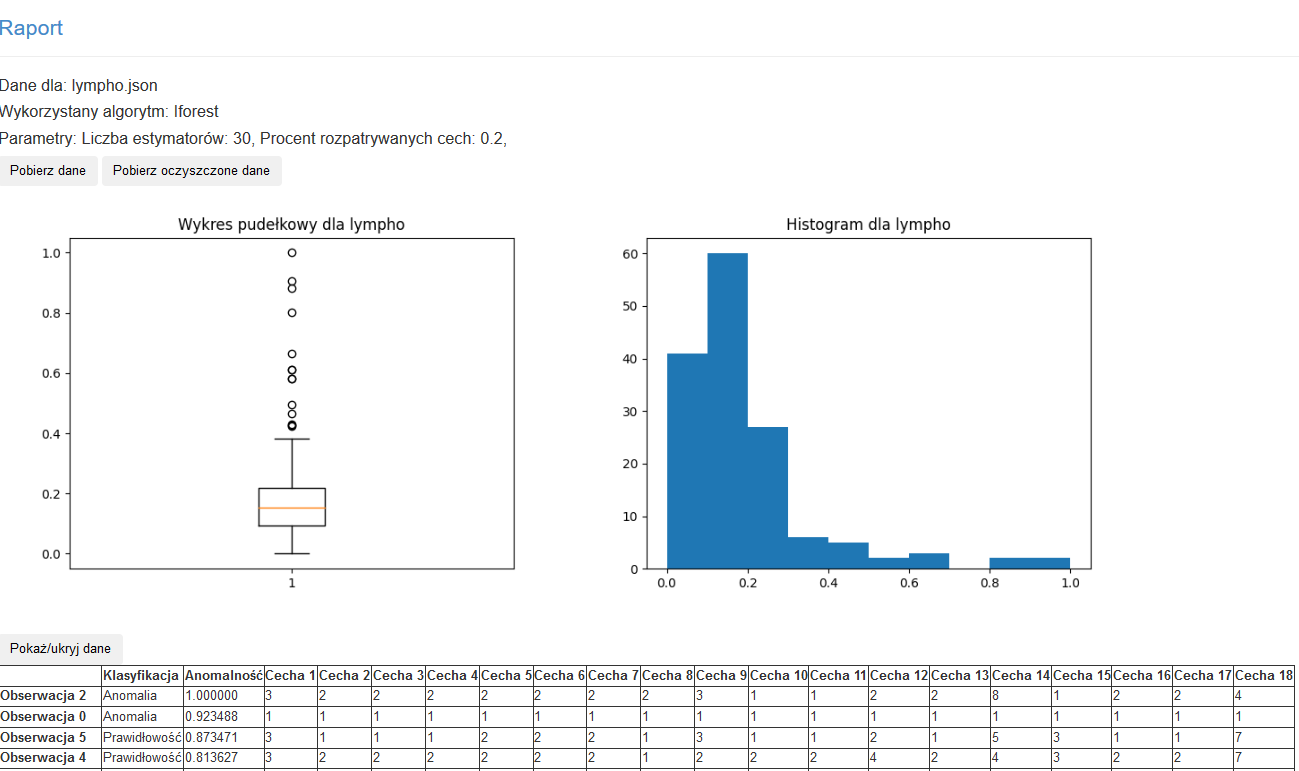
\includegraphics[width = \textwidth]{chapters/projekt/images/Screenshot_2021-01-29 Raport(3).png}
  \caption{Strona systemu po skończeniu zadania detekcji anomalii}
  \footnotesize{źródło: Opracowanie własne}
  \label{fig:label}
 \end{sidewaysfigure}
